\documentclass{article}
	
\usepackage[margin=1in]{geometry}		% For setting margins
\usepackage{amsmath}				% For Math
\usepackage[]{amssymb}
\usepackage{amsmath}
\usepackage{gensymb}
\usepackage{fancyhdr}				% For fancy header/footer
\usepackage{graphicx}				% For including figure/image
\usepackage{cancel}					% To use the slash to cancel out stuff in work
\usepackage{wasysym}                % For cent symbol
\usepackage{needspace}              % To force item to next page
\usepackage{mathtools}

%%%%%%%%%%%%%%%%%%%%%%
% Set up fancy header/footer
\pagestyle{fancy}
\fancyhead[RO,R]{{\large\textbf{PHYS-102}}}
\fancyhead[LO,L]{\large{\textbf{Ch 33 Problem Set}}}
% \fancyhead[CO,C]{\large{\textbf{Part 1}}}
% \fancyhead[RO,R]{\today}
\fancyfoot[LO,L]{}
\fancyfoot[CO,C]{\thepage}
\fancyfoot[RO,R]{}
\renewcommand{\headrulewidth}{0.4pt}
\renewcommand{\footrulewidth}{0.4pt}
%%%%%%%%%%%%%%%%%%%%%%

\newcommand{\hmwkTitle}{Chapter 33 Lenses and Optical Instruments}
% \newcommand{\hmwkDueDate}{February 12, 2014}
\newcommand{\hmwkClass}{PHYS-102}
% \newcommand{\hmwkClassTime}{}
% \newcommand{\hmwkClassInstructor}{Professor Isaac Newton}
\newcommand{\hmwkAuthorName}{\textbf{\underline{\hspace{3in}}}}

% math shortcuts
\newcommand\rr{\quad\Rightarrow\quad}
\newcommand{\spc}{\vspace{1em}\hrule\vspace{1em}}
\newcommand{\bp}[1]{\left(#1\right)}
\newcommand{\bb}[1]{\left[#1\right]}

%
% Title Page
%

\title{
    \vspace{2in}
    \textmd{\textbf{\hmwkTitle}}\\
    \vspace{0.5in}
    \textmd{\textbf{\hmwkClass}}\\
    % \normalsize\vspace{0.1in}\small{Due\ on\ \hmwkDueDate\ at 3:10pm}\\
    % \vspace{0.1in}\large{\textit{\hmwkClassInstructor\ \hmwkClassTime}}
    \vspace{4in}
}

\author{\hmwkAuthorName}
\date{}
\begin{document}
\maketitle
\newpage
\begin{center}
    \section*{\textbf{\underline {Conceptual Questions}}}
\end{center}
\subsubsection*{
    1. Where must the film be placed if a camera lens is to make a sharp image
    of an object far away?
}
The film must be places behind the lens at the focal length of the lens.
\subsubsection*{
    3.  Can a diverging lens form a real image under any circumstances? Explain. 
}
By itself, no, because by definition a diverging lens causes light rays to
diverge which will not bring the rays to a focus point required for a real image.
However, with the combination of a "stronger" converging lens, we can bring the
rays to a focus point to form a real image.
\subsubsection*{
    8. Compare the mirror equation with the thin lens equation. Discuss similarities
    and differences, especially the sign conventions for the quantities involved.
}
The mirror equation and the lens equation are identical. According to the sign conventions, d > 0
indicates a real object or image and d < 0 indicates a virtual object or image, for both mirrors and
lenses. But the positions of the objects and images are different for a mirror and a lens. For a mirror,
a real object or image will be in front of the mirror and a virtual object or image will be behind the
mirror. For a lens, a real image will be on the opposite side of the lens from a real object, and a
virtual image will be on the same side of the lens as the real object.
\subsubsection*{
    14. The thicker a double convex lens is in the center as compared to its edges,
    the shorter its focal length for a given lens diameter. Explain.
}
A double convex lens causes light rays to converge because the
light bends towards the normal as it enters the lens and away
from the normal as it exits the lens. The result, due to the
curvature of the sides of the lens, is that the light bends towards
the principal axis at both surfaces. The more strongly the sides of
the lens are curved, the greater the bending, and the shorter the
focal length.
\begin{figure}[h]
    \begin{center}
        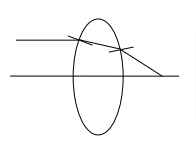
\includegraphics[width=0.3\textwidth]{figures/q14.png}
    \end{center}
\end{figure}
\subsubsection*{
    19. You can tell whether people are nearsighted or farsighted by looking at the
    width of their fa e through their glasses. If a person’s face appears narrower
    through the glasses, is the person farsighted or nearsighted? 
}
\begin{figure}[h]
    \begin{center}
        
\includegraphics[width=0.3\textwidth]{figures/q19.jpg}
    \end{center}
\end{figure}
Nearsighted. Diverging lenses are used to correct nearsightedness and converging lenses are used to
correct farsightedness. If the person’s face appears narrower through the glasses, then the image of
the face produced by the lenses is smaller than the face, virtual, and upright. Thus, the lenses must be
diverging, and therefore the person is nearsighted.
\subsubsection*{
    20. The human eye is much like a camera - yet, when a camera shutter is left open
    and the camera is moved, the image will be blurred. But when you move your head
    with your eyes open, you still see clearly. Explain.
}
All light entering the camera lens while the shutter is open contributes to a single picture. If the
camera is moved while the shutter is open, the position of the image on the film moves. The new
image position overlaps the previous image position, causing a blurry final image. With the eye, new
images are continuously being formed by the nervous system, so images do not “build up” on the
retina and overlap with each other.
\subsubsection*{
    26. For both converging and diverging lenses discuss how the focal length
        from red light differs from that for violet light 
}
For both converging and diverging lenses, the focal point for violet light is closer to the lens than the
focal point for red light. The index of refraction for violet light is slightly greater than for red light
for glass, so the violet light bends more, resulting in a smaller magnitude focal length.
\newpage
\begin{center}
    \section*{\textbf{\underline {Problems}}}
    \subsection*{\textbf{\textit{33-1 and 33-2 Thin Lenses}}}
\end{center}
\subsubsection*{
    1. A sharp image is located 373 mm behind a 215 mm focal length converging lens.
    Find the object distance (a) using a ray diagram, (b) by calculation.
}
\begin{figure}[h]
    \begin{center}
        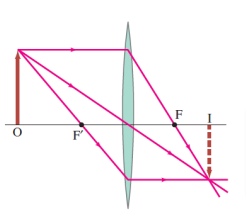
\includegraphics[width=0.3\textwidth]{figures/p1.png}
    \end{center}
\end{figure}
\begin{align*}
    \intertext{(a)}
    \Aboxed{&\approx 480 cm}
    \intertext{(b) Converging lens so $f$ is positive, real image so $d_i$ is
    positive, negative height so image is inverted}
    \frac 1 {d_o}  &= \frac 1 f - \frac 1 {d_i} \\
    d_0 &= \frac{fd_i}{d_i - f} = \frac{(215\;mm)(373\;mm)}{373\;mm - 215\;mm} \\
    \Aboxed{d_o &\approx 508\;mm}
\end{align*}
\subsubsection*{
    2. Sunlight is observed to focus at a point 18.5 cm behind a lens, (a) What kind
    of lens is it? (b) What is its power in diopters?
}
\begin{align*}
    \intertext{(a) Converging lens since it is focused at a point behind the
    lens}
    \intertext{(b) Let $P = \frac 1 f$ (\textit{$f$ for and abject at infinity =
    $F$})}
    P &= \frac 1 {0.185\;m} \\
    \Aboxed{P &\approx 5.41D}
\end{align*}
\subsubsection*{
    4. A certain lens focuses an object 1.85 m away as an image 48.3 cm on the other
    side of the lens. What type of lens is it, and what is its focal length?
    Is the image real or virtual?
}
\begin{align*}
    \intertext{Converging lens and the image is real}
    \frac 1 f &= \frac 1 {d_o} + \frac 1 {d_i} \\
    f &= \frac{d_o d_i}{d_i - d_o} = \frac{(1.85\;m)(0.483\;m)}{0.483\;m - 1.85\;m} \\
    \Aboxed{f &\approx 0.382\;m}
\end{align*}
\subsubsection*{
    6. A stamp collector uses a converging lens with focal length 28 cm to view a stamp
    18 cm in front of the lens. (a) Where is the image located? (b) What is the magnification?
}
\begin{align*}
    \intertext{(a)}
\end{align*}
\subsubsection*{
    10. (a) How far from a 50.0 mm focal length lens must an object be placed if its image
    is to be magnified 2.50X and be real? (b) What if the image is to be virtual and magnified 2.50X?
}
\subsubsection*{
    12. (a) A 2.80 cm-high insect is 1.30 m from a 135 mm focal length lens. Where is the image,
    how high is it, and what type is it? (b) What if f = -135 mm?
}
\subsubsection*{
    13. A bright object and a viewing screen are separated by a distance of 86.0 cm. At what location(s)
    between the object and the screen should a lens of focal length 16.0 cm be placed in order to produce
    a sharp image on the screen? [Hint, first draw a diagram.]
}
\subsubsection*{
    14. How far apart are an object and an image formed by an 85 cm focal length converging lens if the
    image is 2.95X larger than the object and is real?
}
\newpage
\begin{center}
    \subsection*{\textbf{\textit{33-3 Lens Combinations}}}
\end{center}
\subsubsection*{
    20. A diverging lens with f = 33.5 cm is placed 14.0 cm behind a converging lens with f = 20.0 cm.
    Where will an object at infinity be focused?
}
\subsubsection*{
    21. Two 25.0 cm focal length converging lenses are placed 16.5 cm apart. An object is placed 35.0 cm
    in front of one lens. Where w ill the final image formed by the second lens be located? What is the
    total magnification?
}
\subsubsection*{
    26. A diverging lens is placed next to a converging lens of
focal length $f_C$, as in Fig. 33 15. If $f_T$ represents the focal
length of the combination, show that the focal length of the
diverging lens, $f_D$, is given by
\[
    \displaystyle\frac{1}{f_D} = \displaystyle\frac{1}{f_T} -
    \displaystyle\frac{1}{f_C}
\]
}

\subsubsection*{
    27. A lighted candle is placed 36 cm in front of a converging lens of focal length $f_1$ = 13 cm,
    which in turn is 56 cm in front of another converging lens of focal length $f_2$ = 16 cm. (a) Draw a 
    ray diagram and estimate the location and the relative size of the final image. (b) Calculate 
    the position and relative size of the final image.
}
\begin{figure}[h]
    \begin{center}
        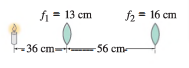
\includegraphics[width=0.3\textwidth]{figures/p27.png}
    \end{center}
\end{figure}
\newpage
\begin{center}
    \subsection*{\textbf{\textit{33-4 Lensmaker's Equation}}}
\end{center}
\subsubsection*{
    28. A double concave lens has surface radii of 33.4 cm and 28.8 cm. What is the focal length if n = 1.58
}
\subsubsection*{
    29. Both surfaces of a double convex lens have radii of 31.4 cm. If the focal length is 28.9 cm, what is
    the index of refraction of the lens material?
}
\subsubsection*{
    33. A prescription for a corrective lens calls for +3.50 diopters. The lensmaker grinds the lens from a
    “blank” with n = 1.56 and convex front surface of radius of curvature of 30.0 cm. What should be the radius
    of curvature of the other surface?
}
\newpage
\begin{center}
    \subsection*{\textbf{\textit{33-6 Eye and Corrective Lenses}}}
\end{center}
\subsubsection*{
    41. A person struggles to read by holding a book at arm’s length, a distance of 55 cm away. What power of
    reading glasses should be prescribed for her, assuming they will be placed 2.0 cm from the eye, and she
    wants to read at the “normal” near point of 25 cm?
}
\subsubsection*{
    42. Reading glasses of what power are needed for a person whose near point is 105 cm, so that he can read
    a computer screen at 55 cm? Assume a lens-eye distance of 1.8 cm.
}
\subsubsection*{
    45. A person’s right eye can see objects clearly only if they are between 25 cm and 78 cm away, (a) What
    power of contact lens is required so that objects far away are sharp? (b) What w ill be the near point
    with the lens in place? 
}
\subsubsection*{
    46. A person has a far point of 14 cm. What power glasses would correct this vision if the glasses were
    placed 2.0 cm from the eye? What power contact lenses, placed on the eye, would the person need?
}
\subsubsection*{
    48. What is the focal length of the eye lens system when viewing an object (a) at infinity, and (b) 38 cm
    from the eye? Assume that the lens retina distance is 2.0 cm.
}
\newpage
\begin{center}
    \subsection*{\textbf{\textit{33-8 Telescopes}}}
\end{center}
\subsubsection*{
    60. What is the magnification of an astronomical telescope whose objective lens has a focal length of 78 cm,
    and whose eyepiece has a focal length of 2.8 cm? What is the overall length of the telescope when adjusted
    for a relaxed eye?
}
\subsubsection*{
    63. An astronomical telescope has an objective with focal length 75 cm and a +35 D eyepiece. What is the
    total magnification?
}
\newpage
\begin{center}
    \subsection*{\textbf{\textit{General Problems}}}
\end{center}
\subsubsection*{
    87. A small object is 25.0 cm from a diverging lens. A converging lens with a focal length of 12.0 cm is
    30.0 cm to the right of the diverging lens. The two lens system forms a real inverted image 17.0 cm to the
    right of the converging lens. What is the focal length of the diverging lens?
}
\begin{figure}[h]
    \begin{center}
        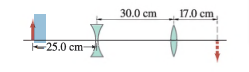
\includegraphics[width=0.3\textwidth]{figures/p87.png}
    \end{center}
\end{figure}

\end{document}
